% Speaker-embedding and change-score sensitivity at Nepali-English code-switch points (IEEEtran conference format).
% Build: pdflatex main && bibtex main && pdflatex main && pdflatex main
% arXiv source package: paper/arxiv/make_arxiv.sh
\documentclass[conference]{IEEEtran}
\IEEEoverridecommandlockouts

\usepackage{cite}
\usepackage{amsmath,amssymb}
\usepackage{graphicx}
\usepackage{booktabs}
\usepackage{array}
\usepackage{url}
\usepackage[utf8]{inputenc}
\usepackage[T1]{fontenc}
\usepackage[hidelinks]{hyperref}
\hypersetup{pdftitle={Speaker-Embedding and Change-Score Sensitivity at Nepali\textendash English Code-Switch Points},
  pdfauthor={Ishan Gautam}}

\begin{document}

\title{Speaker-Embedding and Change-Score Sensitivity\\
at Nepali--English Code-Switch Points}

\author{%
\IEEEauthorblockN{Ishan Gautam}
\IEEEauthorblockA{Pulchowk Campus, Institute of Engineering\\
Pulchowk, Lalitpur\\
Tribhuvan University, Nepal\\
\texttt{isangautam@gmail.com}}
}

\maketitle

\begin{abstract}
People who code-switch change language mid-utterance without changing identity. We ask
whether, within one speaker, speaker-embedding similarity drops and a speaker-change
score rises across a Nepali--English switch. In a pre-registered analysis of real speech, we compare
same-speaker windows straddling a switch with matched same-language controls, for three
speaker embeddings, over 17 YouTube channels (a proxy for speakers). The pre-registered
tests of whether this reaches a full diarization pipeline could not be run. Between
language runs of at least 1~s, similarity is lower across a switch for all three embeddings
and in every channel ($d_z$ $0.19$--$0.27$), and cross-language same-speaker scores are
$0.17$--$0.22$ SD lower; for one embedding both estimates are below our smallest effects of
interest. A two-window change score shows a small excess only where both language runs last
at least $1$~s (AUC $0.57$--$0.58$), a primary cell we chose after seeing results on three
separate pilot channels. Averaged over all switches there is no excess (AUC $\approx 0.49$).
No result reverses with any one channel left out (post hoc). For two embeddings the excess
survives channel-level adjustment for measured acoustic covariates, but the observational
design cannot show that language causes it. On Hindi-- and Bengali--English (MUCS~2021) the
direction is the same, but its speaker IDs are tutorials, not verified speakers. Two of
three pre-registered mitigations could be tested. Their reductions of the excess
($18.9\%$ and $24.9\%$) are inconclusive (Holm $p=0.20$ and $0.70$), no larger than a
non-significant score offset's, at unmeasured cost in missed speaker changes. In a post hoc check, two off-the-shelf diarization pipelines reported a speaker change at
4 and 1 of 300 natural switches, against 1 of 300 matched controls (not significant). The evidence is preliminary: no independent listener has checked the
switch points.
\end{abstract}

\begin{IEEEkeywords}
speaker embeddings, speaker diarization, speaker change detection, code-switching, Nepali,
cross-lingual speaker verification, language identification, pre-registration
\end{IEEEkeywords}

\section{Introduction}
\label{sec:intro}
Speaker diarization relies on speaker embeddings and on scores that compare adjacent
windows. If a language switch by one speaker (SS-DL: \emph{same speaker, different
language}) moves the embedding, a diarization system could report a speaker change that
is not there. We test the first link of that chain. Is same-speaker embedding similarity lower, and a two-window change score higher, at natural Nepali$\leftrightarrow$English switches than at matched same-language boundaries of the same speaker? And do the two testable pre-registered mitigations reduce that excess? In short: between
language runs of at least a second, same-speaker similarity is slightly but consistently
lower across a switch and the change score slightly higher; averaged over all switches, most
of which border a run shorter than half a second, there is no change-score excess, and
neither testable mitigation demonstrably removed the excess. Two kinds of
pre-registered test could not be run. One asks whether the excess survives segmentation,
clustering and temporal smoothing in a full diarization system. The other asks whether a
mitigation makes a system miss real cross-lingual speaker turns (DS-DL: \emph{different
speaker, different language}). Both need
long-form audio and conversations with language-labelled turns, which we could not obtain
(\S\ref{sec:data-conv}). The only pipeline-level evidence here is a post hoc, exploratory
check with two off-the-shelf pipelines on D1 clips and artificial clip joins
(\S\ref{sec:pipe}). The paper is therefore a diagnostic study of embedding and
change-score sensitivity, not an evaluation of diarization error.

That speaker embeddings rate the same speaker as less similar across languages is known from cross-lingual verification~\cite{thienpondt2022,li2026} and, for synthetic Indic voices, from LASE~\cite{menta2026lase}.
DISPLACE reports aggregate diarization error on code-mixed
conversations~\cite{baghel2023displace}. Our contribution is narrower. We measure the shift
\emph{at individual, natural switch points} in real speech, against matched same-speaker
controls, for Nepali--English. We did not find a prior study at this boundary level.

We did not assume the answer. LASE found that the cross-script gap of off-the-shelf
encoders shrinks for Indian-accented (synthetic) voices~\cite{menta2026lase}, so for
speakers whose first language is Nepali the effect may be small. We pre-registered the
study so that a small or null effect could still be reported. The sample, 17 confirmatory
channels, was fixed by the data, not chosen for power. The pre-registration gives the power of this fixed sample at the smallest
effects of interest, from pilot variance components at their upper 80\% bound: 0.68--1.00 for
the similarity test (H1) and 0.70--0.76 for the change-score test (H2-P0) across the three
embeddings. We grade each claim with two labels. An excess measured at switch points is
\emph{switch-associated}. It is \emph{covariate-robust} if it survives channel-level
adjustment for measured acoustic covariates and phrase-boundary controls, and the
non-adjacent embedding test (H3) agrees. The pre-registration calls this grade
``language-attributable''. Because the design is observational, it shows an association
that remains after adjustment for the measured covariates, not that language causes the
excess.

\noindent\textbf{Contributions.}
\begin{itemize}
  \item A boundary-level protocol that compares speaker-embedding similarity and a
        two-window change score at same-speaker language switches with matched
        same-language controls, adjusted for measured acoustic covariates.
  \item Pre-registered results on real Nepali--English speech for three speaker
        embeddings and the change score (\S\ref{sec:results}). The change-score excess
        appears only where both language runs last at least a second, a cell chosen as
        primary after the pilot, and is small there; averaged over all switches there is
        no excess.
  \item A pre-registered check of direction on Hindi-- and Bengali--English
        (\S\ref{sec:h7}), whose speaker labels are unverified.
  \item A pre-registered, inconclusive test of two mitigations against the switch-point
        excess (\S\ref{sec:mitigations}). Neither is supported or does better than a language-aware score offset (itself not significant), and the adversarial one made the embedding more, not less, language-decodable, so the test does not address language invariance.
  \item An exploratory, post hoc check with two off-the-shelf diarization pipelines
        (\S\ref{sec:pipe}). Natural switches rarely produced a false speaker change, not
        significantly more often than matched same-language boundaries.
\end{itemize}
Code, pre-registration and results are at
\href{https://github.com/ishangautam7/nepali-cs-diarization}{\nolinkurl{github.com/ishangautam7/nepali-cs-diarization}}.

\section{Related Work}
\label{sec:related}
\textbf{Code-switching.}
Linguistic work distinguishes the insertion of single words or constituents into a matrix
language from alternation between longer stretches of two languages~\cite{poplack1980,muysken2000}.
Do\u{g}ru\"{o}z et al.~\cite{dogruoz2021survey} survey code-switching for language technologies,
and the code-mixing index (CMI) measures how mixed a text is~\cite{gamback2016cmi}. Our
switch points include both kinds, and most are insertion-like (\S\ref{sec:discussion}).

\textbf{Cross-lingual speaker representations.}
Speaker embeddings underestimate same-speaker similarity when the two utterances are
in different languages, and probing shows that they also encode spoken content and
channel~\cite{raj2019probing}. Thienpondt et al.~\cite{thienpondt2022} describe this score shift and
correct it with language information. More recent work removes language with subspace
normalisation~\cite{hosseini2026} or gradient-reversal adversarial
training~\cite{menta2026lase,li2026}. Hosseini-Kivanani~\cite{hosseini2026} and Li et al.~\cite{li2026} evaluate verification only. Li et al.\ apply the adversarial loss on real multilingual speech (TidyVoiceX); adding TTS speech to their full real training set did not improve verification, although they suggest it may help when real data are scarce. LASE~\cite{menta2026lase} trains on TTS-generated
cross-script pairs. Besides verification, it reports a synthetic code-switched diarization
benchmark: 50 conversations concatenated from 2--4 TTS voices, one of which may switch
language. Segments and the number of speakers are given, and it reports the adjusted Rand
index and cross-script recall. LASE also reports that the cross-script gap of off-the-shelf encoders is smaller for synthetic Indian-accented voices (0.006 vs.\ 0.082 for WavLM-SV; 0.044 vs.\ 0.105 for ECAPA-TDNN). This is why we treat a small or null effect as a real
possibility. Our H1 and H3 therefore measure a known phenomenon on a new language pair. What
is new is where we measure it: at individual natural switch points in real speech,
against matched same-speaker controls.

\textbf{Neural diarization.}
Modern systems combine a powerset segmentation model~\cite{plaquet2023} with
embedding clustering. DiariZen pairs WavLM-based segmentation with WeSpeaker
embeddings and VBx-style clustering~\cite{han2025diarizen,landini2022vbx}, and
DiaPer uses perceiver attractors~\cite{landini2024diaper}. We do not know of an evaluation
of these systems at within-speaker language switches.

\textbf{Code-mixed and low-resource diarization.}
The DISPLACE challenges~\cite{baghel2023displace,displace2024} report aggregate
diarization error on multilingual Indian conversations, and DISPLACE-M extends this
to code-switched medical speech~\cite{displacem2026,barahona2026}. The closest
Nepali work trains multilingual diarizers and evaluates them on Nepali--Hindi
speech~\cite{neupane2026}. These studies report corpus-level error on real conversations.
None of them, nor LASE's synthetic benchmark, reports embedding similarity or a change score at individual natural switch points.

\textbf{Language vs.\ speaker change.}
Mishra and Prasanna~\cite{mishra2023} detect spoken-language change by analogy with speaker-change
detection, which suggests that the two are acoustically entangled. Our acoustic covariates
and phrase-boundary controls (\S\ref{sec:method}) address part of this entanglement.

\section{Data}
\label{sec:data}
\subsection{D1: Nepali--English code-switching corpus (diagnostic)}
We use a Nepali--English code-switched corpus of STEM lectures~\cite{dahal2026csasr},
with its revision pinned in the release. It has 20{,}805 clips (58.4~h) from 161
source videos across 20 YouTube channels, at 16~kHz and loudness-normalised.\footnote{Data-set labels follow the pre-registration; D2 and D3 were the planned conversation sets (\S\ref{sec:data-conv}).} Its transcripts
are mostly machine-generated; 777 clips (586 train, 23 validation, 168 test) are
human-verified, so language tags and switch points inherit transcription errors, which the
listening check (\S\ref{sec:results}) bounds for the primary cell. The
dataset's \texttt{speaker\_id} is the \emph{channel}, not a verified person, and one
channel may carry more than one voice. We therefore run a per-video speaker-purity audit
(\S\ref{sec:method}) and report a purity-audited subset as a sensitivity analysis. We use
only the real (non-augmented) split. The 3 validation channels are the pilot, used to fix
all thresholds. The confirmatory analysis then runs once on the 17 remaining channels (15
training and 2 test), pre-registered and frozen before any confirmatory statistic is
computed.

\subsection{D4: MUCS 2021 Hindi/Bengali--English (direction check)}
For a pre-registered check of direction (H7), we use the MUCS~2021 code-switched
subsets~\cite{diwan2021mucs}: Hindi--English (52{,}825 train and 3{,}136 test clips) and
Bengali--English (26{,}606 and 4{,}275), cut from narrated computer-science spoken
tutorials. The MUCS authors state that speaker information was not available, and that
their speaker counts assume each tutorial has a different speaker~\cite{diwan2021mucs}. In
our copy every speaker ID covers one recording, except one Hindi ID that covers two. A MUCS
``speaker'' is therefore a tutorial, and one narrator may appear under many IDs. MUCS often
writes English words in native script, for example the English word ``office'' in
Devanagari. English loans make up $7.1\%$ of Hindi and $4.7\%$ of Bengali native-script
tokens, so a Latin-script rule alone mislabels the language. We therefore build a
per-script lexicon from the frequent native-script word forms. LLM-based labellers, in eight
parallel runs, labelled
each form as loan, native or name. The lexicon has 763 loans and 67 names for Hindi, and
393 and 21 for Bengali, and its candidate review lists cover 97.0\% of Hindi and 94.4\% of
Bengali native-script tokens. A 60-item spot-check found one arguable label, Bengali ``column'' labelled native.
These are text-only checks of the labels, not audio validation. For the two pairs, this gives 5{,}491 (train) / 237 (test) and 3{,}269 / 580
SS-DL switch points eligible for H1 with 1~s windows, of which 4{,}267 and 2{,}769 have matched
controls (3{,}828 and 2{,}582 of these sets fall in tutorials that meet the 5-unit minimum of
\S\ref{sec:h7} and enter the H1 tests), and 5{,}428 / 235 and 3{,}253 / 584 in the primary detection cell
(\S\ref{sec:method}), of which 5{,}071 and 3{,}510 have cell controls.

\subsection{Long-form audio and conversation data (not obtained)}
\label{sec:data-conv}
D1's clips last 3--14~s, too short for the planned tests of segmentation, clustering and
temporal smoothing over a recording, and the long-form
source videos could not be downloaded. The DS-DL (different-speaker, different-language)
side needs conversations with human references for both speaker \emph{and} language. The
pre-registered source was DISPLACE~2024, whose language-diarization track labels the
language of every segment~\cite{displace2024}, with DISPLACE-M~\cite{displacem2026} as the
fallback. We were not granted access to DISPLACE~2024 during the study. DISPLACE-M is also
access-controlled and has no language references. The pre-registered full-pipeline tests,
the DS-DL non-inferiority test (H5), the ordering of the mitigations (H6) and the joint
trade-off were therefore not run. Apart from the artificial
speaker changes of the exploratory check (\S\ref{sec:pipe}), no result in this paper
involves a speaker change.

\section{Method}
\label{sec:method}

\subsection{Switch points, controls and matching}
We romanise each word with uroman~\cite{hermjakob2018uroman}, which restores Devanagari
inherent vowels. We then force-align the clip on the GPU with torchaudio's MMS\_FA bundle
(MMS-300M~\cite{pratap2023mms}), using Whisper~\cite{radford2023whisper} word timestamps only
as a cross-check. We tag each word's language from the transcript script with a loan/name
lexicon, and detect pauses with the Silero VAD~\cite{silero2021vad}. An SS-DL switch point
is the boundary between two adjacent words of the same speaker in different languages. It
needs both boundary words aligned and no neutral or loan word between the two runs, and no
analysis window may contain a neutral or loan word.
Each point goes into a run-length stratum ($<0.5$, $0.5$--$1$, $\geq 1$~s) set by the
shorter adjacent language run. Two analysis families use the points differently. The
\emph{embedding} family (H1) compares each switch point with up to three same-language
control boundaries from the same clip, or else the same video, matched exactly on pause
bin, position bin and context length. They are also
matched, implicitly, on run-length stratum: both runs must last at least a second, which
places every H1 point in the $\geq 1$~s stratum. The \emph{detection} family (H2-P0)
compares the switch points with all same-speaker controls in the same
video~$\times$~pause-bin~$\times$~position-bin cell, standardised per cell. The collar is
$c=0.5$~s. H1's windows end and start at the edges of the pause, so they exclude it; P0's
two 1~s windows meet at the middle of the pause (or at the word boundary if there is none),
so each holds half of any pause. Within each family, switch points and controls are measured
in the same way.

\emph{Primary detection cell.} The primary cell, \texttt{p0L1}, keeps only switch points
where both language runs last at least a second, with a clean $\pm1$~s field. On the confirmatory channels \texttt{p0L1} holds 3{,}962 switch points with cell controls (3{,}851 train and 111 test; 107 more have no control in their cell), compared with 31{,}844 controls in 964 cells, and the pooled cell 120{,}630 (the sum of its run-length strata).

\emph{How the primary cell was chosen.} The study plan, committed before the pilot, pooled all switch points. On the 3 pilot channels the pooled AUC was $0.486$--$0.494$. At $\tau$, switch points between runs of at least 1~s fired at 15--18\% (535 points), against about 7\% below 0.5~s and 10\% at controls; these rates were not standardised by cell and may partly reflect pauses. We first kept the pooled cell, because changing the primary cell after seeing pilot effects could bias the test. On reviewing the pilot, we then named \texttt{p0L1} primary on construct grounds: a detector with 1~s windows cannot register a sub-second insertion as a two-sided change. The cell gives P0 the run-length condition that the study plan had fixed for H1 before the pilot (both runs at least 1~s). The choice was therefore made after pilot outcomes had been seen. The pre-registration was written after this change and names \texttt{p0L1}, and the configuration was frozen before the one confirmatory run. The 17 confirmatory channels are disjoint from the pilot channels as channels (the purity audit suggests one pilot video may share a confirmatory channel's teacher), which protects the test's error rate. The question it tests, however, was chosen with knowledge of pilot outcomes, and on the confirmatory channels it yields a positive result where the original pooled estimand shows no excess. We therefore report both.

\subsection{Systems}
We test three speaker embeddings: E1 ECAPA-TDNN~\cite{desplanques2020ecapa}, E2 the
WeSpeaker ResNet34-LM embedding~\cite{wang2023wespeaker} of pyannote Community-1 (revision
\texttt{3533c8cf}), and E3 WavLM-Large + ECAPA~\cite{chen2022wavlm}. The change score P0
scores each boundary by $d(t)=1-\cos$ between the $1$~s windows before and after it,
computed on a dense grid of positions. Within $\pm c$ of the boundary it keeps the highest
peak (discarding smaller nearby peaks) and reports a change, or \emph{fires}, when that peak
exceeds an operating point $\tau$. We fix $\tau$ on the pilot channels so that $10\%$ of
controls fire. $\Delta$FAR is how much more often P0 fires at switch points than at their matched controls, standardised within each cell. Every fire at a same-speaker boundary is a false alarm, so $\Delta$FAR is a change-score false-alarm excess, not a diarization error rate. P0 is a
transparent probe of what a change detector sees, not a diarization system. In the primary
cell, P0's score at the boundary compares two 1~s windows much like H1's (they meet at the
middle of any pause instead of excluding it),
in a similar population (both runs at least 1~s), so H2-P0's AUC largely restates H1's
similarity drop as a ranking against cell controls; what P0 adds is peak picking and the
operating point ($\Delta$FAR). Full-pipeline
variants (P1: pyannote Community-1 with VBx~\cite{landini2022vbx} or an AHC back end on
E1--E3; P2: DiariZen~\cite{han2025diarizen}) were planned to test whether the excess
survives segmentation and clustering. They were not run (\S\ref{sec:data-conv});
\S\ref{sec:pipe} reports a post hoc check with the released pipelines instead. On the pilot
channels we also built a language-change score: a language-ID model~\cite{valk2021voxlingua} gives language posteriors for the 1~s window on each side of a boundary, and the score is the Jensen--Shannon divergence between them. It scored switch points above cell-matched controls with AUC 0.58 overall and 0.72 where the shorter run lasts at least 1~s. It also scores pause-bearing phrase boundaries above other controls (AUC 0.56), so it is a weak, partly pause-sensitive check that the switch points carry a language change.

\subsection{Speaker-purity audit}
Because \texttt{speaker\_id} is a channel, we audit it with two embedding families that
are not under test (TitaNet-L and CAM++). Each clip is compared only with same-video clips
of similar language mix, defined by speech type $\times$ the channel's tertile of the code-mixing index (CMI)~\cite{gamback2016cmi}, so that a
language-sensitive embedding does not flag English-heavy clips. A clip is flagged when,
under both embeddings, its mean cosine to those clips lies more than 3.5 robust SDs below
the cell median. A video is split off when its centroid is below the 1st percentile of
within-video split-half cosines to every other video of its channel. The audit flagged 688
of 20{,}444 assessable clips (3.4\%), at the same rate in every language-mix stratum
(3.2--3.6\%), and split off 34 of 161 videos. Different videos of one channel typically
have a centroid cosine of 0.77--0.95, so the split-off rule also separates recording
sessions of one teacher. Judged by embedding similarity against the 99.9th percentile of
cross-channel video similarity, six videos look like other speakers, and one pilot-channel
video may share the teacher of a confirmatory channel (that channel is left out in
\S\ref{sec:results}). Apart from that pilot video, the closest pair of videos from two
different channels has a cosine of 0.65/0.66 (TitaNet-L/CAM++), below the 0.77--0.95
typical of two videos of one channel, so the channels appear to be different speakers. With flagged clips dropped and
split-off videos as their own clusters (46 clusters), every primary result keeps its
direction and meets its smallest effect: H1 $d_z$ 0.25/0.21/0.26, H2-P0 AUC 0.58/0.56/0.59
and H3 $-0.24/-0.20/-0.25$ target SD (E1/E2/E3). Because sessions of one teacher then count
as separate clusters, these $p$-values are optimistic, and the subset analysis is
descriptive. A blind listening check covered the first 117 of the 230 planned pairs, in their
randomised order, with one rater, the author, who knew the hypotheses
The main voice of a flagged clip was judged different
from its video's usual speaker in 51\% of the usable pairs (43 of 84; 95\% CI 41--62\%),
against 8\% for control pairs of two unflagged clips (1 of 12; 1--35\%). Of the flagged
pairs, 14\% were unusable. By this check about half of the flagged clips are other voices,
which the subset analysis removes. The audit is embedding-based, and the check is not an
independent human verification of speaker identity. The mixed models are reported on all
clips only (\S\ref{sec:results}).

\subsection{Mitigations}
\label{sec:mit-method}
We pre-registered three mitigations meant to remove language information, and three
baselines to compare them against. The mitigations are M1, a training-free subspace
projection that removes the language direction from the embedding~\cite{hosseini2026}; M2,
a language-ID--gated change score~\cite{valk2021voxlingua}; and M3, gradient-reversal
adversarial fine-tuning~\cite{ganin2015grl} of the embedding on real speech only (no TTS).
The baselines are B0, the unmodified system with its operating point recalibrated; B1,
language-wise mean centring; and B2, a language-aware score offset~\cite{thienpondt2022}.
Each mitigation was to be scored on the SS-DL excess (H4), on DS-DL misses (H5), and on
their ordering (H6: M3 best, M1 smallest gain). Without conversation data
(\S\ref{sec:data-conv}), only H4 can be tested, on D1. M2 cannot be tested even there: its
gate weight was to be tuned on conversations, because on D1, which has no real speaker changes, any gate lowers the fire rate at switch points and its cost in missed speaker changes cannot be seen. M2 therefore keeps its place in H4's Holm family at $p=1$ and is
reported as not tested. A lower SS-DL excess alone is not an improvement, because
H5 could not check the cost in missed real speaker changes.

\emph{H4 design (pre-registered supplement).} The back end is P0 with E3, as in the
diagnostic analysis. The 15 train channels are scored in 5 folds of 3. For each fold, B1's
means, B2's offset and M1's language direction are estimated, and M3 is trained, on the
other 12 channels only. Every operating point $\tau$ is set on the 3 pilot channels to a
10\% control fire rate, and M3 early-stops on them. M3 starts from E3 with WavLM frozen. It
trains on the fold's channels, with flagged clips dropped, plus a Nepali speaker pool from
IndicVoices~\cite{javed2024indicvoices}. It uses AAM-softmax~\cite{deng2019arcface},
supervised-contrastive and gradient-reversal language losses and a distillation term
towards E3 (weight 0.3), with five seeds per fold. The distillation weights 0, 0.1 and 1
and four ablations, each at seed 0, are secondary analyses. For each channel, $\delta_M =
\Delta\mathrm{FAR}_M - \Delta\mathrm{FAR}_{B0}$ on the primary cell (M3 averaged over seeds)
is tested by an exact one-sided sign-flip over channels, with $p$-values Holm-adjusted over M1--M3. Support also
needs a reduction of at least 25\% of B0's excess.

\subsection{Statistics (pre-registered)}
We compute per-cluster statistics with exact sign-flip permutation tests over the 17 D1
confirmatory channels ($2^{17}$ sign patterns) and BCa bootstrap intervals. These tests
treat channels as independent speakers. Holm correction adjusts the tests' $p$-values within hypothesis
families: $m=3$ for H1 and H3, and $m=5$ for H2, where the pre-registered P1 and P2
pipeline tests, which were not run, hold places at $p=1$ (the post hoc check of
\S\ref{sec:pipe} is not these tests). This can only make the reported H2 verdicts more conservative. Holm changes
only $p$-values: the estimates (AUC, $d_z$, SD units) are unadjusted, and their BCa intervals are at the level $1-0.05/m$. On D4,
where clusters number in the hundreds, the sign-flip draws $2^{17}$ random sign patterns, and
$p=(b+1)/(2^{17}+1)$, where $b$ counts the patterns at least as extreme as the observed statistic. H3 is the mean target-score difference (cross-language minus
mono-language) on lag-matched same-speaker trials, in units of each embedding's target-score
SD, tested by the same channel-level sign-flip. For H1, $d_z$ is the mean over channels of
each channel's mean cosine drop (control minus switch), divided by the pooled within-channel
SD of the per-set drops. For H2-P0, a channel's AUC is the probability that a switch point's
$d(t)$ exceeds that of a same-cell control (ties count half), pooled over cells weighted by
switch points; the estimate is the mean over channels. H1 does not balance its controls by
language; H3 weights Nepali--Nepali and English--English trials equally, so it guards
against language-specific score levels. Each primary hypothesis is reported as
\emph{supported}, \emph{significant, below the smallest effect} (pre-registered label:
\emph{nonzero but trivial}), \emph{reversed}, \emph{equivalent} (TOST), or
\emph{inconclusive}. All 17 non-pilot channels are confirmatory, and the 3 validation
channels are the pilot. An excess is \emph{covariate-robust} (pre-registered label: language-attributable) only if four tests are all significant, each at $\alpha=.05$ without further multiplicity adjustment: (i)~the primary test, after Holm correction; (ii)~a channel-level test adjusted for the acoustic covariates; (iii)~a phrase-boundary contrast; and (iv)~the non-adjacent test H3, after Holm correction. The covariate-adjusted test uses F0, energy, speaking rate, spectral tilt and SNR, as left--right changes. The
plan's C50 reverberation proxy was not estimated, because its source, the gated Brouhaha
model, was not accessible. The phrase-boundary contrast repeats the primary test on switch points with a pause $>150$~ms and their controls in the same pause bins, which are same-language phrase boundaries. Unmeasured differences, such as
reverberation or prosodic phrasing that the covariates miss, cannot be excluded, nor can
syntactic position: switch points sit at run edges, which often coincide with syntactic
boundaries, while controls lie inside runs. A logistic
GLMM with the acoustic covariates, pause bin and position is a descriptive sensitivity
model, not the grading rule.

\section{Diagnostic Results: Embeddings and Change Score on D1}
\label{sec:results}
\emph{Confirmatory run on 17 D1 channels with the frozen configuration. Exact sign-flip tests over channels with Holm-adjusted $p$-values; the
estimates are unadjusted, with BCa intervals at $1-0.05/m$.} All nine primary tests are significant (Table~\ref{tab:d1-primary}). Every one of the 17 channels shows the predicted direction for H1 and H2-P0 with all three embeddings, and for H3 with E1 and E3 (16 of 17 with E2). These are not nine independent findings: H1 and H2-P0 compare similar 1~s windows, and H3 uses the same embeddings.

\begin{table}[t]
\caption{D1 primary outcomes (frozen run). Outcomes follow from the Holm-adjusted sign-flip
$p$-values and the smallest effects of interest (SESOI: $d_z\,0.2$, AUC $0.55$, $0.2$ SD); the estimates are unadjusted. BCa CIs
at $1-0.05/m$: $98.3\%$ for H1 and H3 ($m=3$), $99\%$ for H2-P0 ($m=5$). $^\dagger$Significant,
point estimate below the SESOI; the CI includes the SESOI, so a negligible effect is not
established (pre-registered label: nonzero but trivial). H2-P0 uses a primary cell chosen
after the pilot (\S\ref{sec:method}); over all switch points its AUC is 0.485--0.493
(Table~\ref{tab:d1-det}). H1 uses 3{,}695 matched sets (426 switch points unmatched).}
\label{tab:d1-primary}
\centering
\setlength{\tabcolsep}{5pt}
\begin{tabular}{llcl}
\toprule
H & Model & Estimate (CI) & Outcome \\
\midrule
H1 & E1 & $d_z$ 0.271 (0.203--0.348) & supported \\
H1 & E2 & $d_z$ 0.194 (0.135--0.266) & significant$^\dagger$ \\
H1 & E3 & $d_z$ 0.254 (0.198--0.305) & supported \\
H2-P0 & E1 & AUC 0.584 (0.559--0.618) & supported \\
H2-P0 & E2 & AUC 0.573 (0.547--0.604) & supported \\
H2-P0 & E3 & AUC 0.582 (0.564--0.601) & supported \\
H3 & E1 & $-0.215$ SD ($-0.240$--$-0.175$) & supported \\
H3 & E2 & $-0.173$ SD ($-0.204$--$-0.124$) & significant$^\dagger$ \\
H3 & E3 & $-0.203$ SD ($-0.239$--$-0.152$) & supported \\
\bottomrule
\end{tabular}
\end{table}

\begin{table}[t]
\caption{H2-P0 detection. The \texttt{p0L1} AUC column is the primary test's estimate, whose
$p$-value is Holm-adjusted (CIs in Table~\ref{tab:d1-primary}); pooled \texttt{det}, \texttt{det\_w1} and
$\Delta$FAR are secondary and unadjusted. $\Delta$FAR is cell-standardised on \texttt{p0L1}
and averaged over the 17 channels with equal weight (Fig.~\ref{fig:det}). Parenthesised values are exact one-sided sign-flip $p$ over channels, unadjusted.}
\label{tab:d1-det}
\centering
\begin{tabular}{lcccc}
\toprule
Model & p0L1 AUC & pooled det & det\_w1 & $\Delta$FAR at $\tau$ (p) \\
\midrule
E1 & 0.584 & 0.488 & 0.480 & $+2.46$ pp (0.046) \\
E2 & 0.573 & 0.485 & 0.477 & $+2.95$ pp (0.023) \\
E3 & 0.582 & 0.493 & 0.486 & $+2.73$ pp (0.003) \\
\bottomrule
\end{tabular}
\end{table}

The smallest effects of interest are $d_z=0.2$ (H1), AUC $=0.55$ (H2-P0) and
$0.2$ target-score SD (H3). ``Supported'' means significant with a point estimate at least
this large, and ``significant, below the smallest effect'' means significant with a smaller
point estimate. The second grade does not show that the effect is negligible: for E2 both
intervals include the smallest effect (H1 $0.135$--$0.266$; H3 $-0.204$ to $-0.124$). There are three detection cells:
\texttt{p0L1}, the primary cell, where both language runs last $\geq 1$~s with a clean
$\pm 1$~s field; pooled \texttt{det}, all switch points ($\pm 0.5$~s); and \texttt{det\_w1},
all switch points with $\pm 1$~s controls. The detection result is therefore conditional:
the excess appears at switches between runs of at least a second, and not across switches
in general (pooled AUC 0.485--0.493; for E2 the 99\% intervals of both pooled cells lie just below 0.5).

Pre-registered secondary outcomes put the size in context. With 0.5~s windows (21{,}721
matched sets, 17 channels), H1's $d_z$ is 0.13/0.10/0.12 (E1/E2/E3; 98.3\% CIs 0.10--0.16,
0.07--0.14, 0.09--0.14), below the smallest effect of interest; with 1.5~s windows (862 sets,
16 channels) it is 0.34/0.24/0.36. Longer windows admit only longer runs, so window length
and run length are confounded here. In verification terms the shift is 0.6--0.9~pp of EER (6--8\% relative): on H3's
trials the EER is 12.9/9.5/11.4\% for cross-language and 12.2/8.9/10.5\% for
mono-language target trials. At $\tau$, P0 fires at 22--25\% of same-language boundaries
with a pause over 150~ms, at 13--17\% of primary-cell switch points and at 8--12\% of other
controls (channel means, not cell-standardised), so for this detector a pause is a larger
source of within-speaker false alarms than a language switch.

The operating-point excess is small and uneven across channels (Fig.~\ref{fig:det}).
$\Delta$FAR is positive in 9, 12 and 13 of the 17 channels for E1, E2 and E3, and ranges
from $-7.9$ to $+23.2$~pp. Table~\ref{tab:d1-det} reports the pre-registered
equal-weight mean over channels. Weighting each switch point equally instead gives $+0.78$, $+2.00$ and $+1.17$~pp: the largest channel (584 switch points) is negative for all three embeddings, and the largest positive values ($+23.2$, $+15.2$ and $+14.0$~pp) come from channels with only 13 and 39 switch points.

The detection excess is concentrated at longer runs (exploratory stratification). Pooled
\texttt{det} AUC rises from $\approx 0.48$ when the shorter run is $<0.5$~s to $\approx 0.59$
when it is $\geq 1.0$~s. This fits a $1$-second detector being unable to register shorter
insertions, though that reading is exploratory.

After acoustic covariates and phrase-boundary controls, H1 is \emph{covariate-robust}
(all four tests significant; reverberation is not among the measured covariates) for all three embeddings. The H2-P0 excess is covariate-robust for E2 (adjusted coefficient in the predicted direction in 11/17 channels, $p=.031$) and E3 (10/17, $p=.008$), and only switch-associated for E1 (9/17, $p=.079$). For H1 the descriptive mixed model points the same way. It gives a switch
effect of $-0.030/-0.024/-0.031$ in cosine (E1/E2/E3; $|z| \geq 7.3$), hardly changed
without the acoustic covariates ($-0.033/-0.027/-0.034$). The H2-P0 logistic GLMM gives log-odds of $+0.23/+0.31/+0.12$ ($z$ 1.40/1.95/1.15; one-sided $p$ .081/.026/.124). In this descriptive model the excess is therefore weak and, except for E2 one-sided, not significant. E3's fit used the pre-registered fallback structure without the random slope and video level, because the fuller fits were singular.

Two pre-registered sensitivity analyses leave every outcome category unchanged. The first
drops points whose boundary words align with probability below $0.093$, keeping 240{,}915
of 255{,}695 points (H1 $d_z$ 0.25/0.17/0.23, H2-P0 AUC 0.58/0.57/0.58 for E1/E2/E3). The
second leaves out the 2 test channels (H1 $d_z$ 0.25/0.20/0.26, AUC 0.58/0.58/0.58, H3
$-0.21/-0.17/-0.21$ SD). Three more analyses re-extract the switch points with one rule
changed: re-tagging ``I'' and capital ``A'' as English, keeping the low-alignment clips,
and counting loan words in the language they are pronounced in. The boundary pipeline had
to be rebuilt after a compute-host loss, so each variant is
compared with a reference run on the rebuilt, unvaried boundaries. No H2-P0 or H3 category
changes in any of these four runs (AUC 0.57--0.58; H3 does not use the switch points). The
one grade that moves is E2's H1, which sits at its smallest effect of interest throughout.
Its $d_z$ is 0.205 in the reference run and 0.211 and 0.209 in the first and third variants
(supported), but 0.183 with the low-alignment clips kept (significant, below the smallest
effect, as is the frozen 0.194). E1 and E3 stay supported ($d_z$ 0.24--0.28). E2's H1 grade is therefore
borderline, and the frozen verdicts in Table~\ref{tab:d1-primary} stand. The pre-registered
repeat of the attribution models with Brouhaha's SNR and reverberation estimates depended on
access to that gated model. Access was not obtained, so the repeat was not run.

\emph{Leaving out one channel (post hoc, exploratory).} We
re-estimated each main effect 17 times, each time without one confirmatory channel, from the
frozen per-channel statistics. No
estimate changes direction, and every primary test stays significant (one-sided sign-flip
over the remaining 16 channels, unadjusted $p\le3.1\times10^{-5}$). With channels weighted
equally, H1's $d_z$ ranges over 0.254--0.290 (E1), 0.181--0.204 (E2) and 0.245--0.266 (E3),
H2-P0's AUC over 0.567--0.589, always above its smallest effect, and H3 over $-0.224$ to
$-0.167$~SD. E2's H1 and E3's H3, which sit at their smallest effects, cross them in 5 and 4
of the 17 fits. Weighting switch points equally gives slightly smaller values, again with no
change of direction (H1 $d_z$ 0.180--0.267, H2-P0 AUC 0.563--0.585); E2's H1 then crosses
its smallest effect in 3 of the 17 fits. The pooled \texttt{det} AUC stays below
0.5 in every fit (0.482--0.498, from the rebuilt inputs, which reproduce the frozen pooled
AUCs to three decimals). The least stable quantity is E1's channel-averaged operating-point
excess. It rests largely on the smallest channel (13 primary-cell switch points, $\Delta$FAR
$+23$~pp): without that channel it is $+1.17$~pp ($p=.09$). For E2 and E3 it stays between
$+2.0$ and $+3.6$~pp. Leaving out the confirmatory channel that may share a teacher with a
pilot-channel video changes no primary estimate by more than 0.006; that video and the
channel's four videos form the four closest cross-channel pairs in the corpus.

A blind listening check, with the author as the only rater, covered the first 352 of the 450
planned items, in their randomised order. It
found no audible language change at 6.3\% of the primary-cell switch points (95\% CI
2.0--11.6\%), and a different speaker, overlap or noise at none of them. It found a
language change at none of the cell's controls. The marker lay within about 0.1~s of a word
boundary at 82\% (74--89\%). Correcting $\Delta$FAR for this contamination raises it by
about 7\%, to $+2.63/+3.15/+2.91$~pp for E1/E2/E3. This correction is descriptive and
assumes that a mislabelled point fires like the other condition. Fig.~\ref{fig:umap}
illustrates the embedding geometry behind H1/H3.

\begin{figure}[t]
\centering
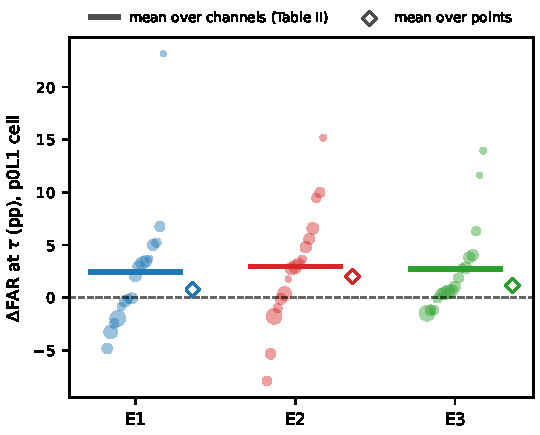
\includegraphics[width=\columnwidth]{figures/delta_far_channels.pdf}
\caption{Change-score excess at the pre-registered operating point on D1 (primary
\texttt{p0L1} cell, 17 confirmatory channels). Each dot is one channel's cell-standardised
$\Delta$FAR: the fire rate at its same-speaker switch points minus that of the matched
same-cell controls (video $\times$ pause $\times$ position), with $\tau$ calibrated to a
$10\%$ control fire rate on the pilot channels. Dot area grows with the channel's number of switch points (13 to 584); horizontal offset within an embedding is by rank only, to reduce overlap. Bars mark the equal-weight mean over channels, the pre-registered
statistic of Table~\ref{tab:d1-det} ($+2.46/+2.95/+2.73$~pp). Diamonds mark the mean over
switch points ($+0.78/+2.00/+1.17$~pp). Single channels vary widely; for E1 the equal-weight
mean rests largely on the smallest channel (13 switch points; \S\ref{sec:results}).}
\label{fig:det}
\end{figure}

\begin{figure}[t]
\centering
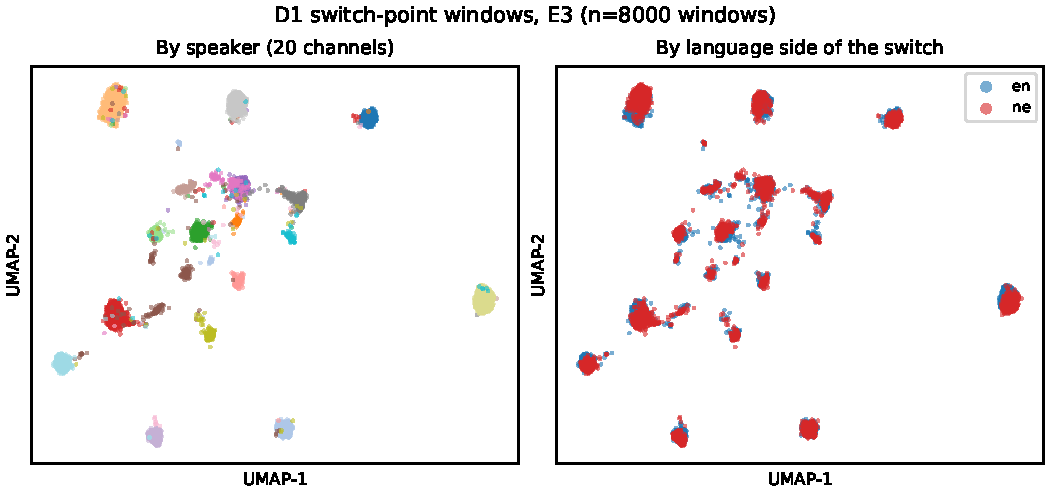
\includegraphics[width=\columnwidth]{figures/umap_speaker_language_invariance.pdf}
\caption{UMAP~\cite{mcinnes2018umap} of D1 switch-point windows (E3, 8000 windows).
\emph{Left:} coloured by channel, our proxy for speaker. Windows cluster by channel: a
linear probe identifies the channel across sessions with balanced accuracy 0.95 (six
channels per fold, chance 0.17). \emph{Right:} coloured by the window's language
($en$/$ne$). The two languages are largely interleaved within each channel, with a small
residual offset consistent with the measured cross-language shift (H1/H3). A linear probe
still recovers the window's language with balanced accuracy 0.76 (chance 0.5). This is a
descriptive illustration, not a test. The probe accuracies come from the H4 secondary
analysis on the clean D1 windows of its five folds, not from the plotted sample.}
\label{fig:umap}
\end{figure}

\section{Direction Check on D4 (Hindi-- and Bengali--English)}
\label{sec:h7}
We repeat the H1 and H2-P0 tests on D4 (MUCS~2021). They were pre-registered and frozen
separately before any D4 outcome was computed.
Clusters are MUCS speaker IDs, that is, tutorials: 364/394 of 550 Hindi IDs and 235/254 of
307 Bengali IDs meet the 5-unit minimum for H1/H2-P0. Holm adjusts the $p$-values of all 12 tests. All
12 are significant in the predicted direction (Holm one-sided $p \le 2.6\times10^{-3}$;
eleven sit at the Monte-Carlo floor). These $p$-values assume that tutorials are independent
speakers. If one narrator recorded many tutorials, the effective number of clusters is
smaller and the $p$-values are too small. The direction matches D1 for both hypotheses and both language pairs: with tutorials as clusters all three embeddings are significant in each cell (pre-registered verdict \emph{replicated}, which counts significance, not size, and treats tutorials as independent speakers). Under voice clusters the verdict in each of the four cells is \emph{not replicated} (see below; Table~\ref{tab:h7}). In
Hindi--English the point estimates are comparable to D1 (D1 H1 $d_z$ $0.19$--$0.27$, AUC
$0.57$--$0.58$), with 2/3 and 3/3 embeddings reaching D1's smallest effect. In
Bengali--English every \emph{point estimate} falls below D1's smallest effect ($0/3$ for
both hypotheses), though some $99.58\%$ intervals still include it. There the direction
matches, but the effect is not shown to reach D1's practical size.

\begin{table}[t]
\caption{H7 on D4 (frozen run), with tutorials (MUCS speaker IDs) as
clusters. All Holm one-sided $p<.05$ in the predicted direction, assuming tutorials are
independent speakers; under the pre-registered voice clusters (6 Hindi, 3 Bengali) none is significant (Holm $p \ge 0.19$ Hindi, $0.88$ Bengali), a test without power (\S\ref{sec:h7}). ``$k$/3'' counts embeddings graded \emph{supported} at D1's smallest
effect ($d_z\,0.2$, AUC $0.55$). CIs are $99.58\%$ BCa.}
\label{tab:h7}
\centering
\footnotesize
\begin{tabular}{llcc}
\toprule
Pair & H & Estimate E1/E2/E3 (CI range) & supported/3 \\
\midrule
hi-en & H1 & $d_z$ 0.24 / 0.18 / 0.26 (.13--.31) & 2/3 \\
hi-en & H2-P0 & AUC 0.56 / 0.56 / 0.58 (.54--.60) & 3/3 \\
bn-en & H1 & $d_z$ 0.16 / 0.12 / 0.15 (.05--.24) & 0/3 \\
bn-en & H2-P0 & AUC 0.53 / 0.52 / 0.54 (.50--.57) & 0/3 \\
\bottomrule
\end{tabular}
\end{table}

The pre-registered voice-cluster sensitivity analysis groups recordings that may share a
narrator. Its outcome-blind threshold, calibrated on D1, collapses the 551 Hindi recordings
to 6 clusters and the 307 Bengali recordings to 3. Under these clusters none of the 12 tests reaches significance (Holm one-sided $p = 0.19$ for five of the six Hindi tests, and $0.88$ for the sixth and for all six Bengali tests). Taken at face value, the pre-registered rule would then label all four verdicts \emph{not robust to speaker dependence}. With only 6 and 3 clusters, however, the test cannot pass: the smallest attainable Holm-adjusted $p$ is $12/2^6 \approx 0.19$, already above $.05$. The non-significance therefore reflects a lack of power, not evidence against the effect, and we report the analysis as uninformative rather than apply that label. Without verified narrator
identities we cannot tell how much of this collapse is over-merging by the threshold and
how much is a small pool of narrators recording many tutorials. We keep the threshold
fixed, since retuning it would break the pre-registration. Robustness to speaker dependence
is therefore \emph{untested} on D4, and the D4 result supports the direction of the effect,
not its significance under realistic speaker dependence.

The pre-registered contamination audit of the native-script lexicon drew 200 random
native-tagged tokens per pair and labelled them with an LLM-based labeller. A second LLM-based check
of 50 per pair agreed on all 100. By these text
labels, English makes up 0.5\% of these tokens in Hindi--English (95\% CI 0.1--2.8\%) and
1.0\% in Bengali--English (0.3--3.6\%). Reading the other 150 Bengali items, outside the
pre-registered check, we found four more English words the labeller had missed:
``column'' and three English stems with Bengali endings (e.g.\ ``line'' with a genitive).
Counting them gives 3.0\% (1.4--6.4\%), probably the fairer reading for Bengali. Neither
check listens to the audio, and we did not quantify how residual mislabelling of this size
affects the D4 estimates. The one
change to code frozen for D4, a crash fix in a descriptive summary made before any D4 result
existed, changes no D1 number and no primary D4 result.

\section{Mitigations}
\label{sec:mitigations}
H4 asks whether M1 and M3 lower the switch-point excess of P0 with E3, compared with the
recalibrated baseline B0, on the 15 scored D1 channels (\S\ref{sec:mit-method}). Support
needs Holm $p<.05$ and a reduction of at least 25\%. The test ran once, from the frozen code, with inputs regenerated by that code after a compute-host loss; an earlier start was cut off before it wrote any output. On these channels
B0's excess is $+2.13$~pp, so the smallest effect of interest is a reduction of 0.53~pp.
Neither mitigation is supported (Table~\ref{tab:h4}). M1 lowers the excess by 0.40~pp
(18.9\%) and M3 by 0.53~pp (24.9\%). Both are \emph{inconclusive}: their intervals include
no reduction at all and are too wide to rule out a reduction of the smallest effect of
interest. M3's point estimate falls just short of the smallest effect of interest (24.9\%
against 25\%), and its per-channel changes vary more than M1's (from $-11.3$ to $+4.1$~pp).
In secondary, unadjusted comparisons, the language-aware score offset B2, which uses predicted window languages, lowers the excess by 0.59~pp ($p=.10$, itself not significant), about as much as either mitigation (M1 $-$ B2: $+0.19$~pp, $p=.67$; M3 $-$ B2: $+0.06$~pp, $p=.54$). Like M2, B2 can lower the switch-point fire rate at no cost visible on D1, so this comparison is biased against the mitigations, and neither B2 nor the mitigations is shown to help without H5. Language-wise centring B1 leaves it unchanged
($+0.09$~pp). H5 (no extra missed cross-lingual turns), H6 (the ordering) and the joint
trade-off are not tested, for lack of conversation data (\S\ref{sec:data-conv}). These
results therefore do not establish a working mitigation.

The pre-registered secondary analyses, all descriptive and unadjusted, help interpret this
null. Linear probes on clean windows show that M1 removes much of the linearly decodable
language information: language balanced accuracy is 0.76 for E3 and 0.62 after M1, while
speaker identification stays at 0.95. Partly removing that information did not detectably
remove the excess. M3, despite its gradient-reversal loss, makes the language \emph{more}
decodable (0.795--0.823 over its five seeds). It also improves verification on the H4 folds'
clean windows, a different trial set from H3's (mono-language EER 0.118 for E3, 0.062--0.071 for M3), and closes the small cross-language
EER gap. So M3 changed the embedding without making it language-invariant, and H4 is not a
test of whether a language-invariant embedding would help. If the fitting folds are allowed
to choose a larger language subspace for M1 ($k=1$--8), the reduction grows to $-0.62$~pp (29\%, unadjusted $p=.004$), but not significantly beyond M1's ($p=.18$), and the larger subspace leaves the language probe where M1 left it (0.62). The reduction is more than random subspaces of the same size give ($p=.008$), but
not clearly more than the top principal directions give ($p=.28$), so it is unclear that the reduction is specific to language. In the pre-registered sensitivity subsets, M1's reduction is
of similar size (purity subset $-0.41$~pp, $p=.02$; alignment filter $-0.43$~pp, $p=.045$),
while M3's vanishes ($+0.80$ and $+0.20$~pp).

M3's secondary variants ran with one seed each (seed 0), so they carry seed noise. The five
seeds of the primary configuration alone range from $-1.05$ to $-0.16$~pp (49\% to 7\%;
standard deviation of the seed means 0.41~pp), and seed 0 is near the strong end
($-0.90$~pp). Without distillation (weight 0), M3 raises the excess ($+0.64$~pp;
$+1.54$~pp against seed 0, 95\% CI $+0.53$ to $+3.31$), and the weights 0.1 and 1 lower it
by 0.31 and 0.21~pp. Dropping the gradient-reversal loss keeps the reduction ($-1.03$~pp;
$-0.12$~pp against seed 0, CI $-0.96$ to $+0.94$). Dropping it together with the
supervised-contrastive loss removes the reduction ($+0.36$~pp; $+1.26$~pp against seed 0,
CI $+0.39$ to $+3.01$). Dropping only the contrastive loss or only the IndicVoices pool
leaves $-0.24$ and $0.00$~pp. Within this noise, the language-adversarial loss does not
seem to be what produces M3's small reduction, which fits the probe result above.

On the two held-out test channels, B0's excess is larger, $+7.22$~pp, and neither
mitigation lowers it consistently. These results are descriptive only: every system was
fitted on all 15 train channels, with M3 as the five all-data models. M3 changes the excess
by $-0.56$~pp on average (from $-1.88$ to $+1.06$~pp over its seeds), and M1 raises it by
2.91~pp. M3 again improves verification (mono-language EER 0.072--0.103 against 0.172 for
E3) without lowering the language probe's accuracy (0.814--0.870 against 0.803).

\begin{table}[t]
\caption{H4 on D1 (frozen run): change in the cell-standardised p0L1 $\Delta$FAR against B0
($+2.13$~pp) over the 15 scored channels; M3 averaged over 5 seeds per fold. Exact one-sided
sign-flip over channels, $p$-values Holm-adjusted over M1--M3; BCa CIs at 98.3\%.}
\label{tab:h4}
\centering
\setlength{\tabcolsep}{4pt}
\begin{tabular}{lcccl}
\toprule
System & Change (pp) & CI (pp) & Holm $p$ & Outcome \\
\midrule
M1 & $-0.40$ (18.9\%) & $-0.98$ to $+0.17$ & 0.20 & inconclusive \\
M2 & --- & --- & 1 & not tested \\
M3 & $-0.53$ (24.9\%) & $-3.89$ to $+0.74$ & 0.70 & inconclusive \\
\bottomrule
\end{tabular}
\end{table}

As a cheap feature-level pre-check, we applied M1 and a language-centring baseline to the
transparent P0 detector on the pilot channels, with the language direction estimated
leave-one-channel-out. There the projection did \emph{not} reduce the p0L1 $\Delta$FAR,
which stayed flat or rose slightly. On 3 pilot channels and without a test, this suggested
that removing a single global language direction from the embedding is not enough by
itself to remove the switch-point excess. The confirmatory test above, on 15 other channels
with the direction fitted fold-wise, agrees: M1's reduction is small and not significant.

\section{Exploratory Full-Pipeline Check (post hoc)}
\label{sec:pipe}
After all pre-registered analyses were complete, we ran two off-the-shelf diarization pipelines as released,
with their default settings and no given number of speakers: pyannote Community-1
(revision \texttt{3533c8cf}, its own VBx clustering~\cite{landini2022vbx}) and
DiariZen~\cite{han2025diarizen} (model \texttt{diarizen-wavlm-large-s80-md}). This check
was not pre-registered, so its tests are exploratory and unadjusted. It is not the planned
P1-AHC variant, whose threshold was to be tuned on conversation data
(\S\ref{sec:data-conv}).

On the 17 confirmatory channels we drew 300 natural \texttt{p0L1} switch points, in
proportion to each channel's count, and one same-cell control for each. Each pipeline ran
on the whole clip that holds the boundary. Because D1 has no speaker changes, we built
artificial ones: 300 joins of a clip from one channel to a clip from another with the same
language at the join, and 300 with a language change. As artificial same-speaker
boundaries, we also joined 300 pairs of consecutive clips from one video, with the same
language at the join. Every side of a join ends or starts with at least 1~s of its
language. A join puts two separately recorded segments end to end, so it also carries a
recording cut: it tests whether a real speaker change is found, not natural turn-taking. A
boundary counts as a speaker change when the pipeline's output switches to a different
speaker within $\pm0.5$~s; silence in between does not count.

\begin{table}[t]
\caption{Exploratory full-pipeline check (post hoc, not pre-registered): share of
boundaries at which the pipeline reports a speaker change within $\pm0.5$~s (300 per row,
17 channels). For one speaker this is a false change; for two speakers, one minus it is the
miss rate. Joins are artificial boundaries. Rates are pooled over boundaries; the differences
in the text are means of per-channel differences.}
\label{tab:pipe}
\centering
\setlength{\tabcolsep}{3pt}
\begin{tabular}{llcc}
\toprule
Boundary & Speakers & Community-1 & DiariZen \\
\midrule
Natural switch (SS-DL) & one & 1.3\% & 0.3\% \\
Natural same-language control & one & 0.3\% & 0.3\% \\
Join, one video, same language & one & 1.7\% & 3.3\% \\
Join, two channels, same language & two & 60.3\% & 94.0\% \\
Join, two channels, language change & two & 65.3\% & 96.0\% \\
\bottomrule
\end{tabular}
\end{table}

Neither pipeline reported a speaker change at natural switch points significantly more
often than at their controls (Table~\ref{tab:pipe}). The mean per-channel differences are $+1.2$~pp for
Community-1 and $-0.4$~pp for DiariZen (two-sided exact sign-flip $p=.31$ and $1.0$ over
17 channels). Both rates are close to zero, so the change-score excess of
Table~\ref{tab:d1-det} did not appear as a detectable excess of false speaker changes in
these two pipelines. The rates rest on 4, 1, 1 and 1 events in 300, and the per-channel
differences have 95\% BCa intervals of $-0.8$ to $+3.6$~pp (Community-1) and $-3.4$ to
$+0.8$~pp (DiariZen). Community-1 also missed 35--40\% of the artificial two-speaker changes
in these short files, so its near-zero rate says little about a subtle effect; DiariZen,
which found 94--96\% of them, gives the more informative null.
Community-1 missed fewer of them when the language also changed (mean per-channel difference
$-9.0$~pp, two-sided $p=.041$, unadjusted; $-5.0$~pp in the pooled rates); for DiariZen the
difference was $-1.5$~pp ($p=.29$). For DiariZen, same-speaker joins drew more false changes than natural
controls ($+6.0$~pp per channel, $p=.031$), as a recording cut would. These tests also treat a channel
as one speaker (\S\ref{sec:data}). The diarization error rates and per-channel values are
in the released repository.

\section{Discussion}
\label{sec:discussion}
Table~\ref{tab:status} summarises what became of each pre-registered test.

\begin{table}[t]
\caption{The pre-registered tests and what became of them.}
\label{tab:status}
\centering
\scriptsize
\setlength{\tabcolsep}{3pt}
\begin{tabular}{@{}l >{\raggedright\arraybackslash}p{0.33\columnwidth} >{\raggedright\arraybackslash}p{0.49\columnwidth}@{}}
\toprule
Test & Question & Status and outcome \\
\midrule
H1 & Same-speaker similarity lower across a switch & Run (\S\ref{sec:results}): supported for E1, E3; significant, below the SESOI for E2 \\
H2-P0 & Change-score excess at switch points & Run in a cell chosen after the pilot: supported for E1--E3; no excess over all switches \\
H2-P1/P2 & The excess in full diarization pipelines & Not run; post hoc check only (\S\ref{sec:pipe}) \\
H3 & Cross-language same-speaker scores lower & Run: as for H1 \\
H4 & Mitigations reduce the excess & M1 and M3 inconclusive; M2 not testable on D1 (\S\ref{sec:mitigations}) \\
H5, H6 & Missed DS-DL turns; ordering of the mitigations & Not run (\S\ref{sec:data-conv}) \\
H7 & Same direction on Hindi/Bengali--English & Run (\S\ref{sec:h7}): replicated with tutorials as clusters; uninformative under voice clusters \\
\bottomrule
\end{tabular}
\end{table}

On real Nepali--English speech, same-speaker embedding similarity is lower across a
language switch (H1), and cross-language same-speaker scores are lower (H3). This confirms,
at natural switch points, the cross-language shift known from
verification~\cite{thienpondt2022,menta2026lase}. For all three embeddings, H1 survives the
pre-registered acoustic and pause controls, and H3 agrees in direction. The shift is therefore not explained by the measured covariates, although
unmeasured ones cannot be excluded. It is small: standardised effects are
$\approx 0.17$--$0.27$, consistent with LASE's report of a reduced cross-script gap for synthetic Indian-accented voices~\cite{menta2026lase}. For the ResNet embedding E2 both effects are significant with point
estimates below our smallest effect of interest, a value their intervals still include. Relative to matched controls, same-speaker cosine drops by 0.037/0.029/0.034 at a switch (E1/E2/E3; H1's channel-mean drop, the numerator of $d_z$). For the ECAPA-TDNN E1 this is close to LASE's off-the-shelf gap for Indian-accented voices (0.044) and well below that for Western-accented voices (0.105); for the WavLM-based E3 it lies between LASE's WavLM-SV gaps (0.006 and 0.082). LASE's gaps are utterance-level, on synthetic voices, and ours come from 1~s windows of real speech, so the comparison is only indicative.

The change score shows a narrower picture. It is higher at switches only where both language runs last at least a second: in the primary cell (AUC $0.57$--$0.58$; covariate-robust
for E2 and E3, switch-associated for E1) and in the $\geq 1$~s stratum of the pooled cell (exploratory). The operating-point excess in the primary cell is
$+2.5$ to $+3.0$~pp averaged over channels (for E1, $+1.2$~pp without its smallest channel; \S\ref{sec:results}), and $+0.8$ to $+2.0$~pp averaged over switch
points. Averaged over all switches, there is no excess (pooled AUC $\approx 0.49$). Most
switches in these lectures are insertion-like~\cite{muysken2000}: in the pooled cell, 79\%
of the 120{,}630 analysed switch points border a run shorter than 0.5~s,
too short for a 1~s detector to resolve. The
short-run stratum has point estimates below $0.5$, which is exploratory and untested. Both
supported claims, H1's and H2-P0's, are therefore conditional on language runs of at least a
second.

The pre-registered tests of whether this reaches diarization output could not be run. In
the exploratory check (\S\ref{sec:pipe}), two off-the-shelf pipelines rarely reported a
speaker change at natural switches, and not significantly more often than at matched
controls; that check used short clips and artificial speaker changes. Whether the same
holds in long-form conversations, and whether a lower false-alarm rate at switches would
cost missed real speaker changes, still needs conversations with speaker and language
references. Nor did the pre-registered
mitigations demonstrably remove the excess. The point estimates for projecting out the language direction and for adversarial fine-tuning were reductions of a fifth to a quarter, but both intervals include no reduction, and neither exceeded that of a language-aware score offset~\cite{thienpondt2022}, which was itself not significant and is favoured on D1 (\S\ref{sec:mitigations}). Because M3 did not become language-invariant, whether invariance
itself would help remains open.

\textbf{Limitations.} Without the pre-registered pipeline tests, whose only stand-in is the
post hoc check on clip joins, the results mainly concern embedding and change-score
sensitivity. The design is
observational, and covariate adjustment covers only the measured covariates. D1's
\texttt{speaker\_id} is a YouTube channel, not a verified identity. The embedding-based
purity audit and a single-rater listening check only partly address this. The
channel-level tests assume that the 17 channels are independent speakers. MUCS speaker IDs
are tutorials, so the D4 tests assume, without verification, that tutorials are
independent speakers. We have no human-verified evaluation subset with checked speaker
continuity, audible switches and boundary timing. One is prepared for two independent
bilingual raters, with its analysis fixed in advance, but not yet labelled, so the
evidence here is preliminary. The listening checks had one rater, the
author, who knew the hypotheses, and the D4 language labels were checked as text by LLMs,
not against the audio. By the listening check, about 6\% of primary-cell switch points
carry no audible switch. D1's transcripts are mostly machine-generated, and the
pre-registered measurement of tag noise on its 777 human-verified clips was not run. Both corpora are instructional monologues (STEM lectures;
narrated tutorials), and we have no speaker metadata such as gender; switching in
conversation, where diarization matters most, may differ in frequency, run length and
prosody. The H4 supplement fixed no power analysis, and its intervals are wider than its smallest effect of interest,
so with 15 channels the test could not separate a 25\% reduction from none. M3 was trained
on real speech only. This avoids the synthetic-to-real mismatch that Li et al.\ suggest may hurt when real data are plentiful~\cite{li2026}, and which LASE, trained and tested on TTS voices only, does not measure. The cost is fewer cross-language training pairs.

\section{Conclusion}
\label{sec:conclusion}
Within one speaker and between language runs of at least a second, three speaker
embeddings rate the same voice as slightly less similar across a natural Nepali--English
switch, and a two-window change score is slightly higher there; averaged over all switches
there is no change-score excess. None of these results reverses when any one channel is left out. The
two mitigations we could test reduced that excess inconclusively.
The evidence is preliminary: channels stand in for speakers, and no independent listener has
yet checked the switch points. Whether the excess reaches diarization output was not tested
as planned; in a post hoc check, two off-the-shelf pipelines rarely reported a false speaker
change at switches. Testing it needs long-form conversations with speaker and language
references.

\section{Ethics and Reproducibility}
\label{sec:ethics}
The study uses real recorded speech only and is a non-commercial project. D1 is used as
released on Hugging Face (CC BY-NC 4.0)~\cite{dahal2026csasr}, MUCS~2021 as released on
OpenSLR (resource 104, CC BY-SA 4.0), and M3's Nepali speaker pool is the Nepali part of
IndicVoices (CC BY 4.0, gated access). No audio is redistributed. Speaker embeddings are
biometric data, so we report only aggregate statistics and release no per-speaker
embeddings. No ethics-board review was sought: the study uses only publicly released
recordings, makes no new recordings and recruits no participants.

Code, configurations, the pre-registration, the decision and deviation logs, data and model
revisions, seeds and all result files are available at
\href{https://github.com/ishangautam7/nepali-cs-diarization}{\nolinkurl{github.com/ishangautam7/nepali-cs-diarization}},
with instructions that map every number in this paper to the command that produced it. Each
confirmatory analysis was frozen as a tagged commit, with the hash of every frozen file,
before it was run, and each result file records the freeze it came from. The pre-registration
was not deposited with an external registry, so its timing rests on the project's own commit
history, which is available on request. The post hoc analyses, added after all
pre-registered results, are marked as exploratory throughout.

\emph{Use of AI tools.} The author designed the study, wrote the pre-registration, made
every analysis decision, ran the listening checks and interpreted the results. AI coding
assistants (Anthropic Claude models) helped write and run analysis code and edit the text,
and LLM-based tools labelled the D4 lexicon and checked the contamination-audit labels as
text (\S\ref{sec:data}, \S\ref{sec:h7}). The author checked their output and is responsible
for all content.

\section*{Conflicts of Interest}
The author declares no conflicts of interest.

\bibliographystyle{IEEEtran}
\bibliography{refs}

\end{document}
